\subsection{System Architecture}
The high‐level design (HLD) of ThermoSight is depicted through the following three diagrams:

\subsubsection{Block Diagram}

As shown in Figure \ref{fig:ts_block}, ThermoSight integrates data acquisition, model inference, and user interfaces into a cohesive pipeline.

\begin{figure}[H]
    \centering
    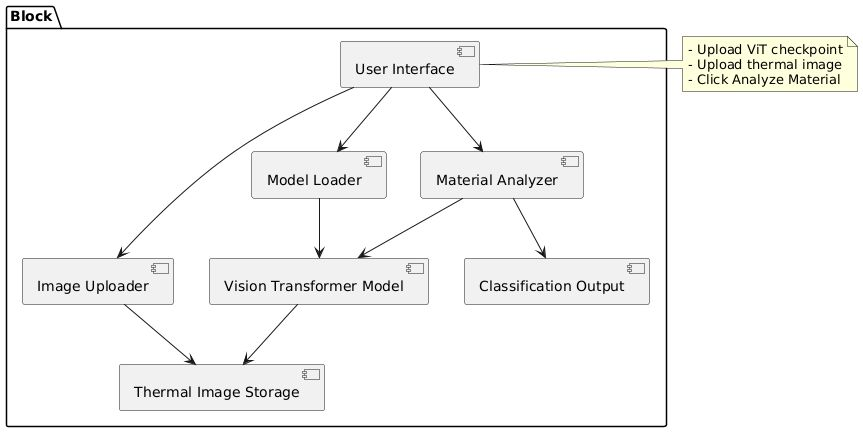
\includegraphics[width=0.9\textwidth]{thermoblock.png}
    \caption{ThermoSight Block Diagram}
    \label{fig:ts_block}
\end{figure}
\medskip

\subsubsection{Component Diagram}

Figure \ref{fig:ts_component} illustrates the main components and their interactions, including the thermal camera, preprocessing module, ViT inference engine, heatmap generator, and user interface.

\begin{figure}[H]
    \centering
    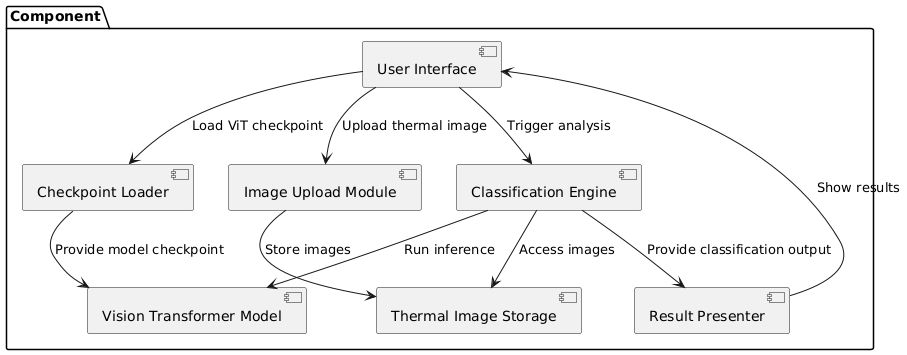
\includegraphics[width=\textwidth]{thermocomponent.png}
    \caption{ThermoSight Component Diagram}
    \label{fig:ts_component}
\end{figure}
\medskip

\subsubsection{Deployment Diagram}

Figure \ref{fig:ts_deployment} shows the Deployment Diagram for ThermoSight, highlighting how the Web/Mobile UI interacts with the server backend, Vision Transformer model, and thermal image storage.

\begin{figure}[H]
    \centering
    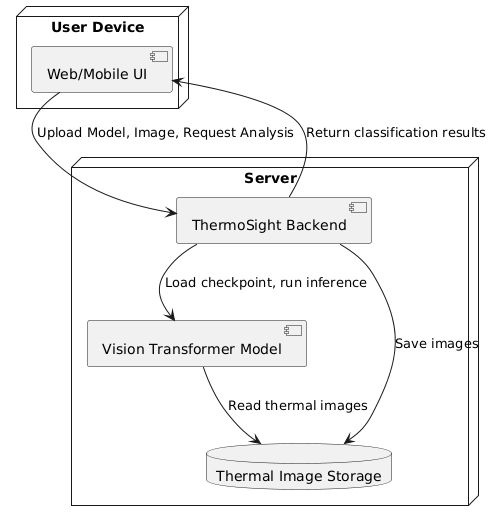
\includegraphics[width=\textwidth]{thermodeployment.png}
    \caption{ThermoSight Deployment Diagram}
    \label{fig:ts_deployment}
\end{figure}
